\chapter{Data Processing Examples}
\label{ch:examples}

\definecolor{lgray}{gray}{0.95}

This chapter showcases a variety of results that are possible when
processing different data sets with the Stereo Pipeline. It is also
a shortened guide that shows the commands and \texttt{stereo.default}
files used to process data. We hope that these are useful templates
that will get you started in processing your own data.

\section{Guidelines for Selecting Stereo Pairs}

When choosing image pairs to process, images that are taken with
similar viewing angles, lighting conditions, and significant surface
coverage overlap are best suited for creating terrain
models. Depending on the characteristics of the mission data set and
the individual images, the degree of acceptable variation will
differ. Significant differences between image characteristics
increases the likelihood of stereo matching error and artifacts, and
these errors will propagate through to the resulting data products.

Although images do not need to be map projected before running the
\texttt{stereo} program, we recommend that you do run {\tt cam2map}
beforehand, especially for image pairs that contain large topographic
variation (and therefore large disparity differences across the
scene, e.g. Valles Marineris).  Map projection is especially necessary
when processing \ac{HiRISE} images. This removes the large disparity
differences between \ac{HiRISE} images and leaves only the small
detail for the Stereo Pipeline to compute. Remember that \ac{ISIS}
can work backwards through a map-projection when applying the camera
model, so the geometric integrity of your images will not be sacrificed
if you map project first.

Excessively noisy images will not correlate well, so images should be
photometrically calibrated in whatever fashion suits your purposes. If
there are photometric problems with the images, those photometric
defects can be misinterpreted as topography.

Remember, in order for \texttt{stereo} to process stereo pairs in
\ac{ISIS} cube format, the images must have had SPICE data associated
by running ISIS's \texttt{spiceinit} program run on them first.

\section{Mars Reconnaissance Orbiter HiRISE}

\ac{HiRISE} is one of the most challenging cameras to use when making 3D
models because \ac{HiRISE} exposures can be several gigabytes each. Working
with this data requires patience as it will take time.

One important fact to know about HiRISE is that it is composed of
multiple linear CCDs that are arranged side by side with some vertical
offsets. These offsets mean that the CCDs will view some of the same
terrain but at a slightly different time and a slightly different
angle. Mosaicking the CCDs together to a single image is not a simple
process and involves living with some imperfections.

One cannot simply use the \ac{HiRISE} RDR products, as they do not
have the required geometric stability.  Instead, the \ac{HiRISE}
EDR products must be assembled using \ac{ISIS} \texttt{noproj}.
The USGS distributes a script in use by the \ac{HiRISE} team that
works forward from the team-produced `balance' cubes, which provides
a de-jittered, noproj'ed mosaic of a single observation, which is
perfectly suitable for use by the Stereo Pipeline (this script was
originally engineered to provide input for SOCET SET).  However,
the `balance' cubes are not available to the general public, and
so we include a program (\texttt{hiedr2mosaic.py}, written in
\href{http://www.python.org}{Python}) that will take \ac{PDS}
available \ac{HiRISE} EDR products and walk through the processing
steps required to provide good input images for \texttt{stereo}.

The program takes all the red CCDs and projects them using the \ac{ISIS}
{\tt noproj} command into the perspective of the RED5 CCD. From there,
{\tt hijitreg} is performed to work out the relative offsets between
CCDs. Finally the CCDs are mosaicked together using the average
offset listed from {\tt hijitreg} using the {\tt handmos} command.
Below is an outline of the processing.

\begin{verbatim}
    hi2isis           # Import HiRISE IMG to Isis
    hical             # Calibrate
    histitch          # Assemble whole-CCD images from the channels
    spiceinit
    spicefit          # For good measure
    noproj            # Project all images into perspective of RED5
    hijitreg          # Work out alignment between CCDs
    handmos           # Mosaic to single file
\end{verbatim}

To use our script, first go to the directory where you have downloaded
the HiRISE's RED EDR \texttt{IMG} files. You can run the 
\texttt{hiedr2mosaic.py} program without any arguments to view a short
help statement, with the \texttt{-h} option to view a longer help statement,
or just run the program on the EDR files like so:

\begin{verbatim}
    hiedr2mosaic.py *.IMG
\end{verbatim}

If you have more than one Obsevation's worth of EDRs in that
directory, then limit the program to just one observation's EDRs
at a time, e.g. \texttt{hiedr2mosaic.py PSP\_001513\_1655*IMG}.  If you
run into problems, try using the \texttt{-k} option to retain all of 
the intermediary image files to help track down the issue.  The
\texttt{hiedr2mosaic.py} program will create a single mosaic file 
with the extension \texttt{.mos\_hijitreged.norm.cub}.  Be warned that
the operations carried out by \texttt{hiedr2mosaic.py} can take many 
hours to complete on the very large HiRISE images.


Finally we recommend map projecting the product and normalizing both
images in the stereo pair using the same dynamic range. Notice that we
map project the second image using the same map settings and crop of
the first image. This means the images will share the same origin and
the {\tt stereo.default} search range can be centered around zero.

\begin{verbatim}
  ISIS 3> cam2map f=first.mos_hijitreged.norm.cub t=first.map.cub
  ISIS 3> cam2map f=second.mos_hijitreged.norm.cub map=first.map.cub \
          to=second.map.cub matchmap=true
  ISIS 3> bandnorm f=first.map.cub t=first.norm.cub
  ISIS 3> bandnorm f=second.map.cub t=second.norm.cub
  ISIS 3> ls first.norm.cub second.norm.cub > fromlist
  ISIS 3> ls first.norm.cub > holdlist
  ISIS 3> equalizer fromlist=fromlist holdlist=holdlist
  ISIS 3> mkdir result
  ISIS 3> stereo first.norm.equ.cub second.norm.equ.cub result/output
\end{verbatim}

In the future, the HiRISE team will be producing de-jittered, noproj'ed
imagery in the \texttt{extras/} directory of their \ac{PDS} volume.
When this happens, most of the above commands will no longer be required,
as you will be able to just run \texttt{cam2map} on their provided imagery.

\subsection{Columbia Hills}

\ac{HiRISE} observations
\href{http://hirise.lpl.arizona.edu/PSP_001513_1655}{PSP\_001513\_1655} and
\href{http://hirise.lpl.arizona.edu/PSP_001777_1650}{PSP\_001777\_1650}
are on the floor of Gusev Crater and cover the area where the \ac{MER} 
Spirit landed and has roved, including the Columbia Hills.

\begin{figure}[h!]
\centering
  \subfigure[{\tt 3D Rendering}]{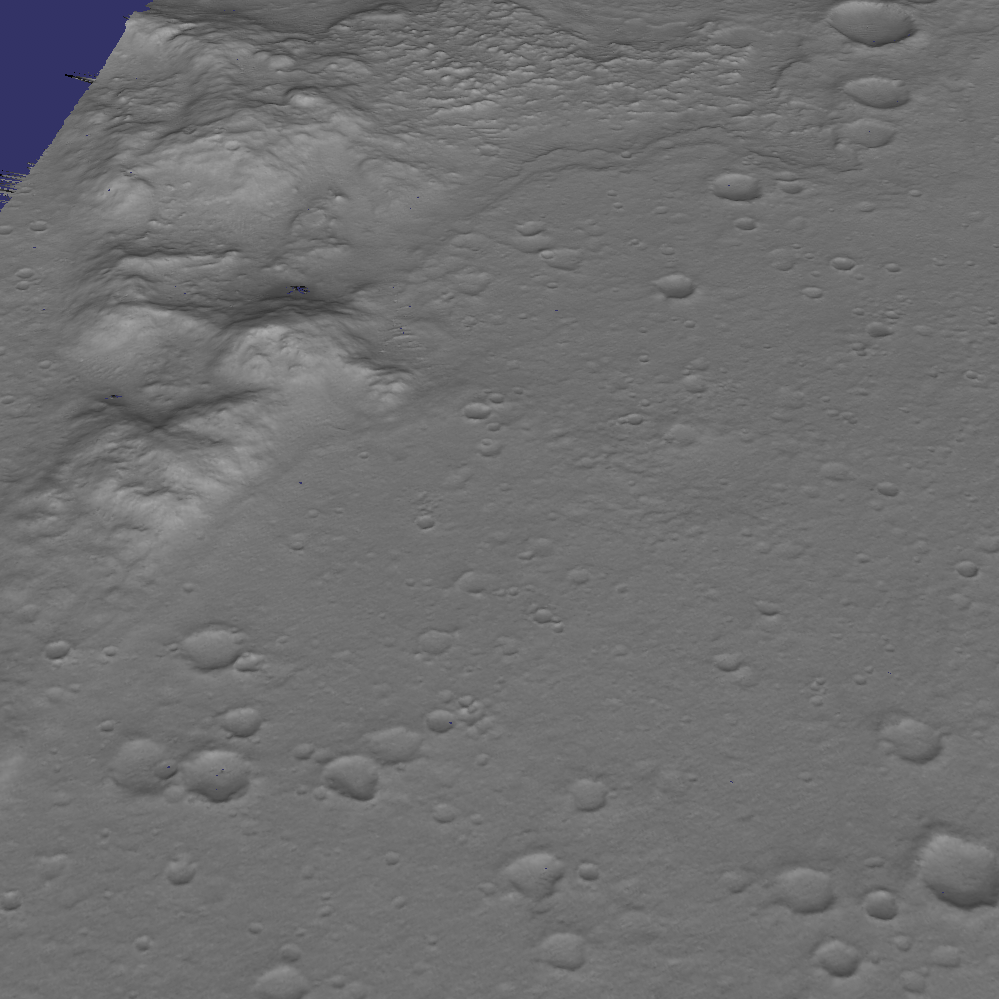
\includegraphics[width=3in]{images/examples/hirise/chills_hirise_example.png}}
  \hfil
  \subfigure[{\tt KML Screenshot}]{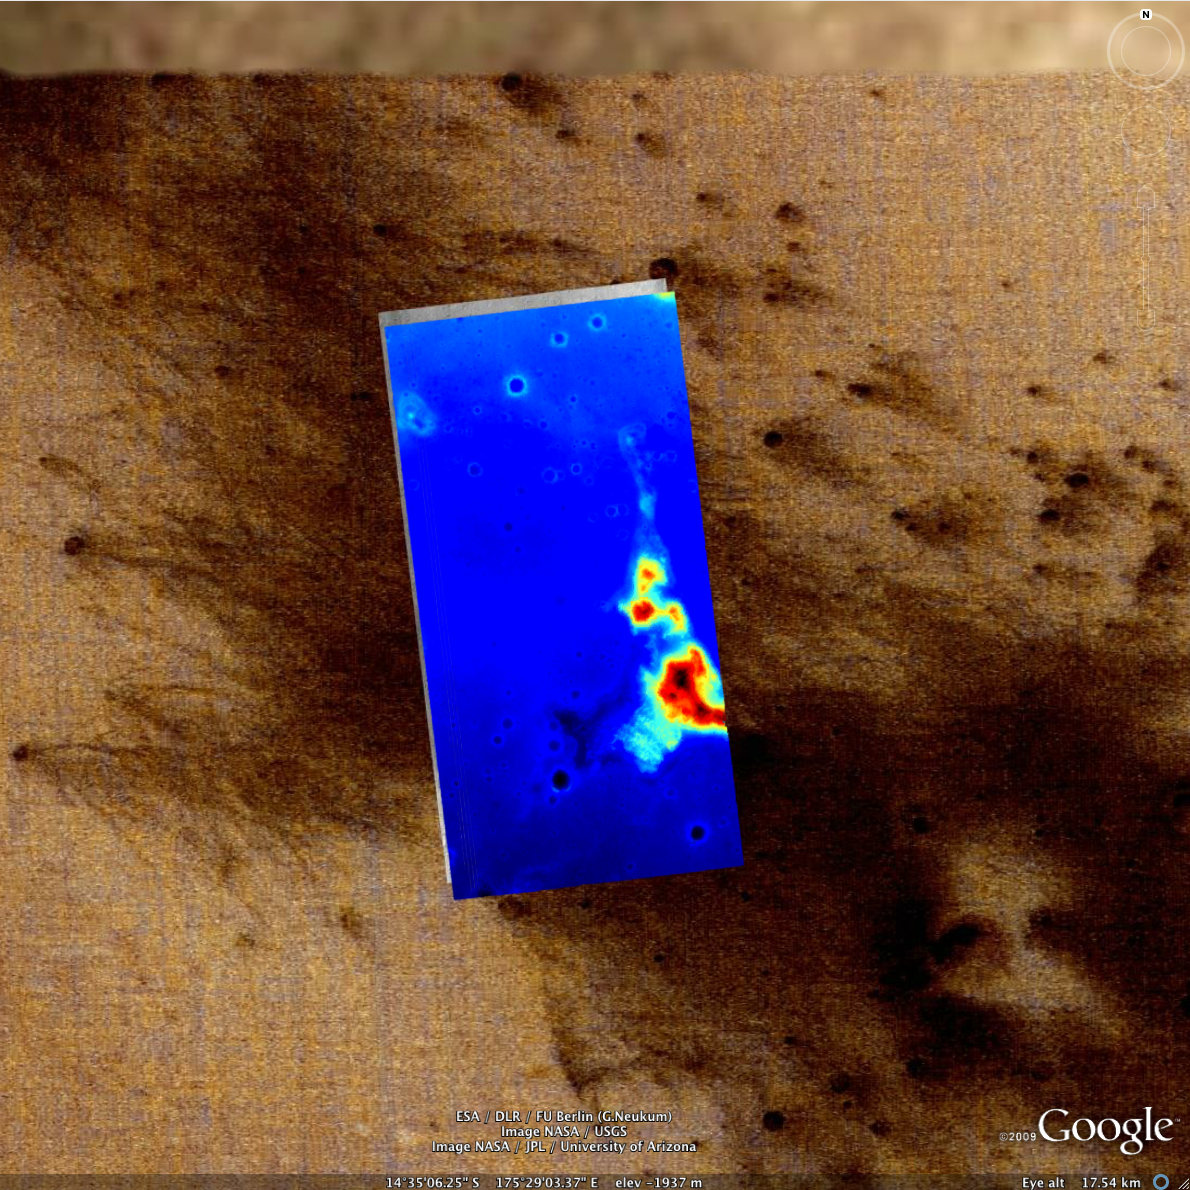
\includegraphics[width=3in]{images/examples/hirise/chills_hirise_ge_example.png}}
\caption{Example output using HiRISE images PSP\_001513\_1655 and
  PSP\_001777\_1650 of the Columbia Hills.}
\label{fig:hirise_chills_example}
\end{figure}

\subsubsection*{Commands}

Download all 20 of the RED EDR \texttt{.IMG} files for each observation.
\begin{verbatim}
  ISIS 3> hiedr2mosaic.py PSP_001513_1655_RED*.IMG
  ISIS 3> hiedr2mosaic.py PSP_001777_1650_RED*.IMG
  ISIS 3> cam2map from=PSP_001513_1655_RED.mos_hijitreged.norm.cub \
                    to=PSP_001513_1655_REDmosaic.map.cub
  ISIS 3> cam2map from=PSP_001777_1650_RED.mos_hijitreged.norm.cub \
                   map=PSP_001513_1655_REDmosaic.map.cub \
                    to=PSP_001777_1650_REDmosaic.norm.cub matchmap=true
  ISIS 3> bandnorm from=PSP_001513_1655_REDmosaic.map.cub \
                     to=PSP_001513_1655_REDmosaic.map.norm.cub
  ISIS 3> bandnorm from=PSP_001777_1650_REDmosaic.map.cub \
                     to=PSP_001777_1650_REDmosaic.map.norm.cub
  ISIS 3> ls *.map.norm.cub > fromlist
  ISIS 3> ls *1513*.map.norm.cub > holdlist
  ISIS 3> equalizer fromlist=fromlist holdlist=holdlist
  ISIS 3> rm *REDmosaic.map.norm.cub *REDmosaic.map.cub
  ISIS 3> mkdir result
  ISIS 3> stereo PSP_001513_1655.map.norm.equ.cub \
                 PSP_001777_1650.map.norm.equ.cub result/output
\end{verbatim}

\subsubsection*{stereo.default}

\begin{center}\begin{minipage}{5.5in}
\begin{Verbatim}[frame=single,fontsize=\small,label=stereo.default for HiRISE Columbia Hills]
    ### PREPROCESSING

    DO_INTERESTPOINT_ALIGNMENT 0
    INTERESTPOINT_ALIGNMENT_SUBSAMPLING 0
    DO_EPIPOLAR_ALIGNMENT 0

    FORCE_USE_ENTIRE_RANGE 1
    DO_INDIVIDUAL_NORMALIZATION 0

    PREPROCESSING_FILTER_MODE 2

    SLOG_KERNEL_WIDTH 1.5

    ### CORRELATION

    COST_MODE 0
    COST_BLUR 0

    H_KERNEL 50
    V_KERNEL 50

    H_CORR_MIN 210
    H_CORR_MAX 450
    V_CORR_MIN -320
    V_CORR_MAX 320

    SUBPIXEL_MODE 2

    SUBPIXEL_H_KERNEL 25
    SUBPIXEL_V_KERNEL 25

    ### FILTERING

    FILL_HOLES 1

    RM_H_HALF_KERN 5
    RM_V_HALF_KERN 5
    RM_MIN_MATCHES 60 # Units = percent
    RM_THRESHOLD 3
    RM_CLEANUP_PASSES 1

    ### DOTCLOUD

    NEAR_UNIVERSE_RADIUS 0.0
    FAR_UNIVERSE_RADIUS 0.0
\end{Verbatim}
\end{minipage}\end{center}

\subsection{East Mareotis Tholus}

\ac{HiRISE} observations
\href{http://hirise.lpl.arizona.edu/PSP_001760_2160}{PSP\_001760\_2160} and
\href{http://hirise.lpl.arizona.edu/PSP_001364_2160}{PSP\_001364\_2160} 
cover East Mareotis Tholus, a small volcano in Tempe Terra.

\begin{figure}[h!]
\centering
  \subfigure[{\tt 3D Rendering}]{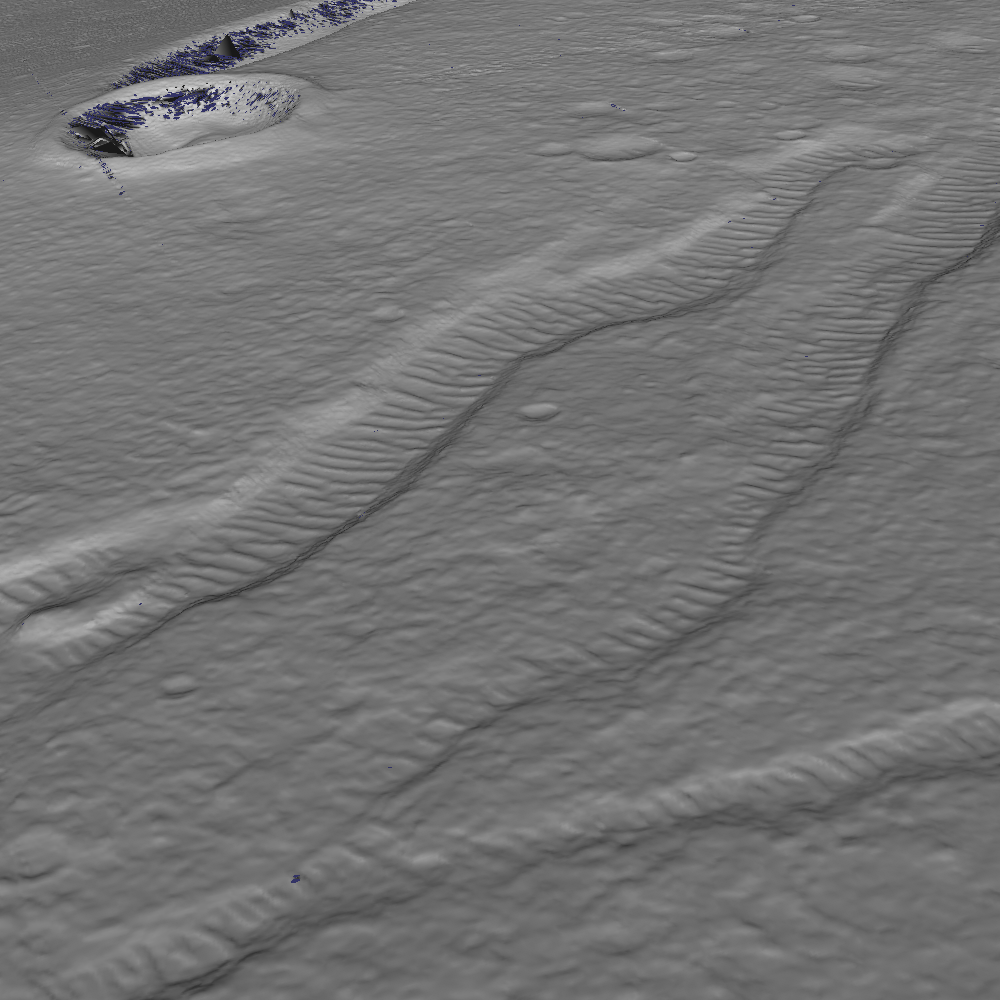
\includegraphics[width=3in]{images/examples/hirise/emare_example.png}}
  \hfil
  \subfigure[{\tt KML Screenshot}]{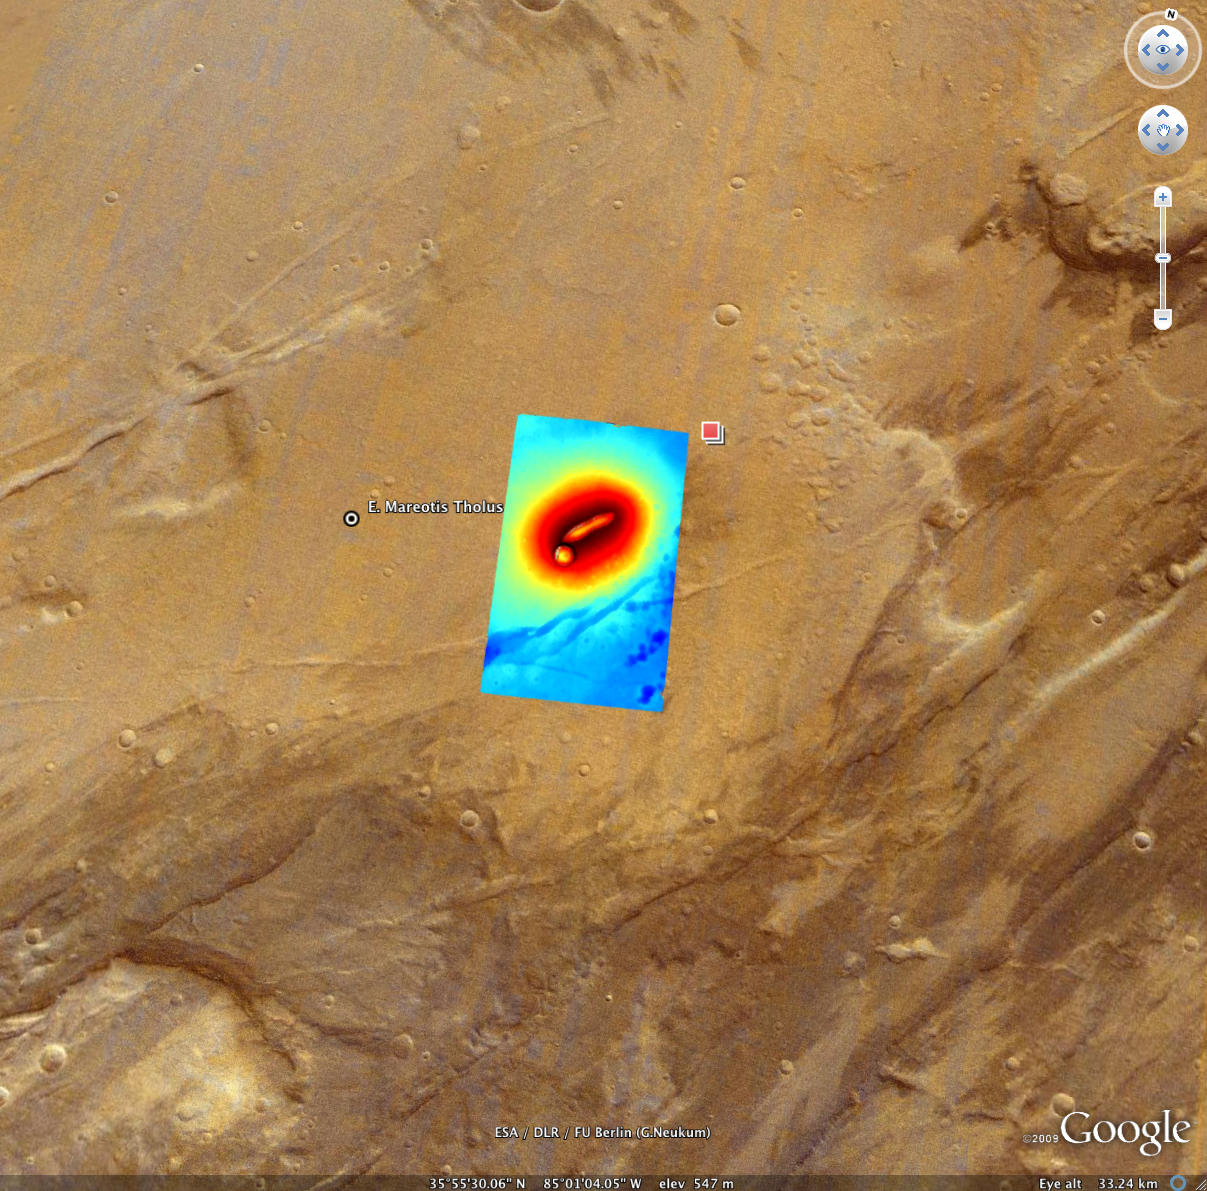
\includegraphics[width=3in]{images/examples/hirise/emare_ge_example.png}}
\caption{Example output using HiRISE images PSP\_001364\_2160 and
  PSP\_001760\_2160 of East Mareotis Tholus.}
\label{fig:hirise_emare_example}
\end{figure}

\subsubsection*{Commands}

Download all 20 of the RED EDR \texttt{.IMG} files for each observation.
\begin{verbatim}
  ISIS 3> hiedr2mosaic.py PSP_001364_2160_RED*.IMG
  ISIS 3> hiedr2mosaic.py PSP_001760_2160_RED*.IMG
  ISIS 3> cam2map from=PSP_001364_2160_RED.mos_hijitreged.norm.cub \
                    to=PSP_001364_2160_REDmosaic.map.cub
  ISIS 3> cam2map from=PSP_001760_2160_RED.mos_hijitreged.norm.cub \
                   map=PSP_001364_2160_REDmosaic.map.cub \
                    to=PSP_001760_2160_REDmosaic.map.cub matchmap=true
  ISIS 3> bandnorm from=PSP_001364_2160_REDmosaic.map.cub \
                     to=PSP_001364_2160_REDmosaic.map.norm.cub
  ISIS 3> bandnorm from=PSP_001760_2160_REDmosaic.map.cub \
                     to=PSP_001760_2160_REDmosaic.map.norm.cub
  ISIS 3> ls *.map.norm.cub > fromlist
  ISIS 3> ls *1760*.map.norm.cub > holdlist
  ISIS 3> equalizer fromlist=fromlist holdlist=holdlist
  ISIS 3> rm *REDmosaic.map.norm.cub *REDmosaic.map.cub
  ISIS 3> mkdir result
  ISIS 3> stereo PSP_001364_2160.map.norm.equ.cub \
                 PSP_001760_2160.map.norm.equ.cub result/output
\end{verbatim}

\subsubsection*{stereo.default}

\begin{center}\begin{minipage}{5.5in}
\begin{Verbatim}[frame=single,fontsize=\small,label=stereo.default for HiRISE East Mareotis Tholus]
    ### PREPROCESSING

    DO_INTERESTPOINT_ALIGNMENT 0
    INTERESTPOINT_ALIGNMENT_SUBSAMPLING 0
    DO_EPIPOLAR_ALIGNMENT 0

    FORCE_USE_ENTIRE_RANGE 1
    DO_INDIVIDUAL_NORMALIZATION 0

    PREPROCESSING_FILTER_MODE 2

    SLOG_KERNEL_WIDTH 1.5

    ### CORRELATION

    COST_BLUR 0
    COST_MODE 0

    H_KERNEL 25
    V_KERNEL 25

    H_CORR_MIN -80
    H_CORR_MAX 150
    V_CORR_MIN -80
    V_CORR_MAX 50

    SUBPIXEL_MODE 0

    SUBPIXEL_H_KERNEL 25
    SUBPIXEL_V_KERNEL 25

    ### FILTERING

    FILL_HOLES 1

    RM_H_HALF_KERN 5
    RM_V_HALF_KERN 5
    RM_MIN_MATCHES 60 # Units = percent
    RM_THRESHOLD 3
    RM_CLEANUP_PASSES 1

    ### DOTCLOUD

    NEAR_UNIVERSE_RADIUS 0.0
    FAR_UNIVERSE_RADIUS 0.0
\end{Verbatim}
\end{minipage}\end{center}

\subsection{North Terra Meridiani Crop}

\ac{HiRISE} observations
\href{http://hirise.lpl.arizona.edu/PSP_001981_1825}{PSP\_001981\_1825} and
\href{http://hirise.lpl.arizona.edu/PSP_002258_1825}{PSP\_002258\_1825}
show a small crater filled by layered material.

\begin{figure}[h!]
\centering
  \subfigure[{\tt 3D Rendering}]{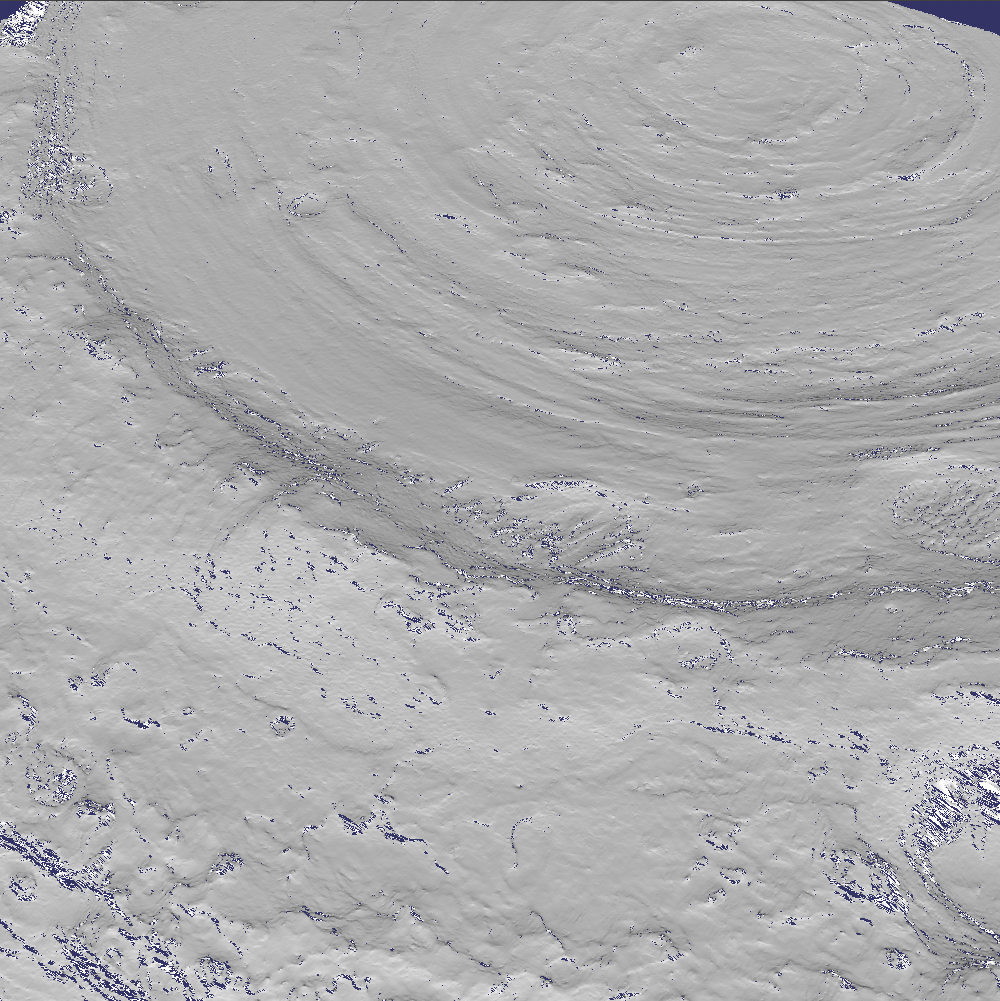
\includegraphics[height=2.5in]{images/examples/hirise/nterra_example.png}}
  \hfil
  \subfigure[{\tt KML Screenshot}]{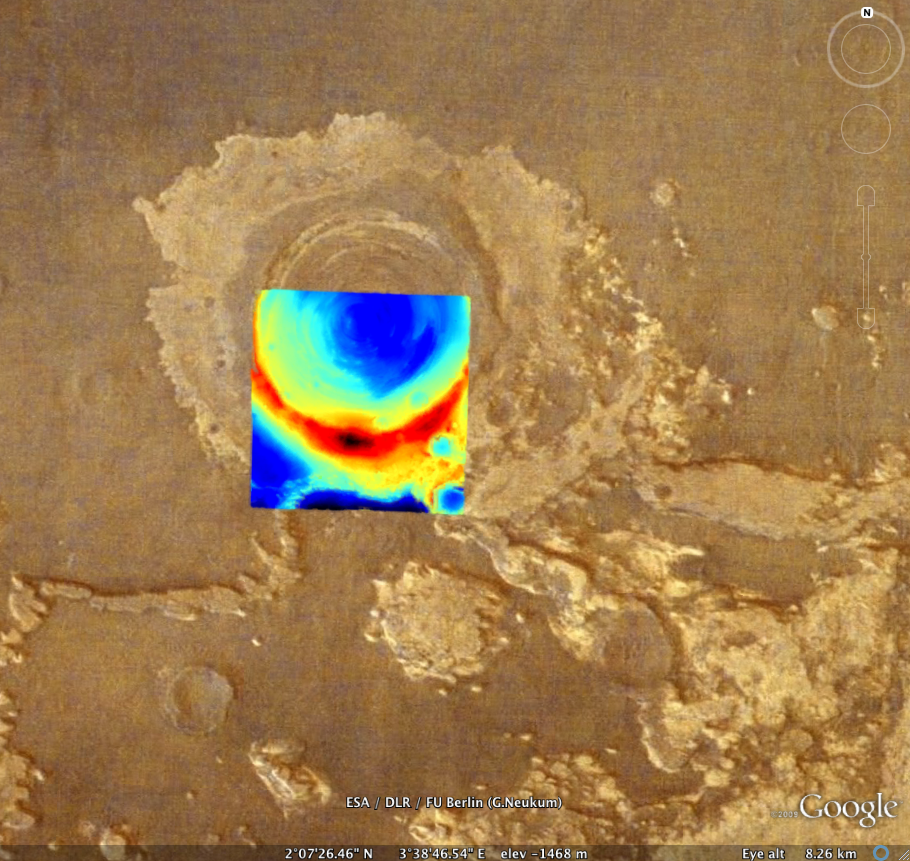
\includegraphics[height=2.5in]{images/examples/hirise/nterra_ge_example.png}}
\caption{Example output using cropped HiRISE data of North Terra Meridiani.}
\label{fig:hirise_nterra_example}
\end{figure}

\subsubsection*{Commands}

Notice here that we have applied a crop to select a subset of these
HiRISE images that we are interested in.  Cropping is often an
efficient way to go because it greatly reduces the amount of
computation necessary to get results in a limited area.  As always,
Download all 20 of the RED EDR \texttt{.IMG} files for each observation.
\begin{verbatim}
  ISIS 3> hiedr2mosaic.py PSP_001981_1825_RED*.IMG
  ISIS 3> hiedr2mosaic.py PSP_002258_1825_RED*.IMG
  ISIS 3> cam2map from=PSP_001981_1825_RED.mos_hijitreged.norm.cub \
                    to=PSP_001981_1825_REDmosaic.map.cub
  ISIS 3> cam2map from=PSP_002258_1825_RED.mos_hijitreged.norm.cub \
                   map=PSP_001981_1825_REDmosaic.map.cub \
                    to=PSP_002258_1825_REDmosaic.map.cub matchmap=true
  ISIS 3> bandnorm from=PSP_001981_1825_REDmosaic.map.cub \
                     to=PSP_001981_1825_REDmosaic.map.norm.cub
  ISIS 3> bandnorm from=PSP_002258_1825_REDmosaic.map.cub \
                     to=PSP_002258_1825_REDmosaic.map.norm.cub
  ISIS 3> ls *.map.norm.cub > fromlist
  ISIS 3> ls *1981*.map.norm.cub > holdlist
  ISIS 3> equalizer fromlist=fromlist holdlist=holdlist
  ISIS 3> crop from=PSP_001981_1825_REDmosaic.map.norm.equ.cub \
                 to=PSP_001981_1825.crop.cub sample=7497 line=41318 nsamp=10000 nline=10000
  ISIS 3> crop from=PSP_002258_1825_REDmosaic.map.norm.equ.cub \
                 to=PSP_002258_1825.crop.cub sample=7982 line=41310 nsamp=10000 nline=10000
  ISIS 3> rm *REDmosaic*.cub
  ISIS 3> mkdir result
  ISIS 3> stereo PSP_001981_1825.crop.cub \
                 PSP_002258_1825.crop.cub result/output
\end{verbatim}

\subsubsection*{stereo.default}

\begin{center}\begin{minipage}{5.5in}
\begin{Verbatim}[frame=single,fontsize=\small,label=stereo.default for HiRISE North Terra Meridiani Crop]
    ### PREPROCESSING

    DO_INTERESTPOINT_ALIGNMENT 0
    INTERESTPOINT_ALIGNMENT_SUBSAMPLING 0
    DO_EPIPOLAR_ALIGNMENT 0

    FORCE_USE_ENTIRE_RANGE 1
    DO_INDIVIDUAL_NORMALIZATION 0

    PREPROCESSING_FILTER_MODE 2

    SLOG_KERNEL_WIDTH 1.5

    ### CORRELATION

    COST_BLUR 21
    COST_MODE 2

    H_KERNEL 45
    V_KERNEL 45

    H_CORR_MIN -270
    H_CORR_MAX -70
    V_CORR_MIN -14
    V_CORR_MAX 26

    SUBPIXEL_MODE 0

    SUBPIXEL_H_KERNEL 25
    SUBPIXEL_V_KERNEL 25

    ### FILTERING

    FILL_HOLES 1

    RM_H_HALF_KERN 5
    RM_V_HALF_KERN 5
    RM_MIN_MATCHES 60 # Units = percent
    RM_THRESHOLD 3
    RM_CLEANUP_PASSES 1

    ### DOTCLOUD

    NEAR_UNIVERSE_RADIUS 0.0
    FAR_UNIVERSE_RADIUS 0.0
\end{Verbatim}
\end{minipage}\end{center}

\vfill

\section{Mars Reconnaissance Orbiter CTX}

\subsection{North Terra Meridiani}

\begin{figure}[b!]
\centering
  \subfigure[{\tt 3D Rendering}]{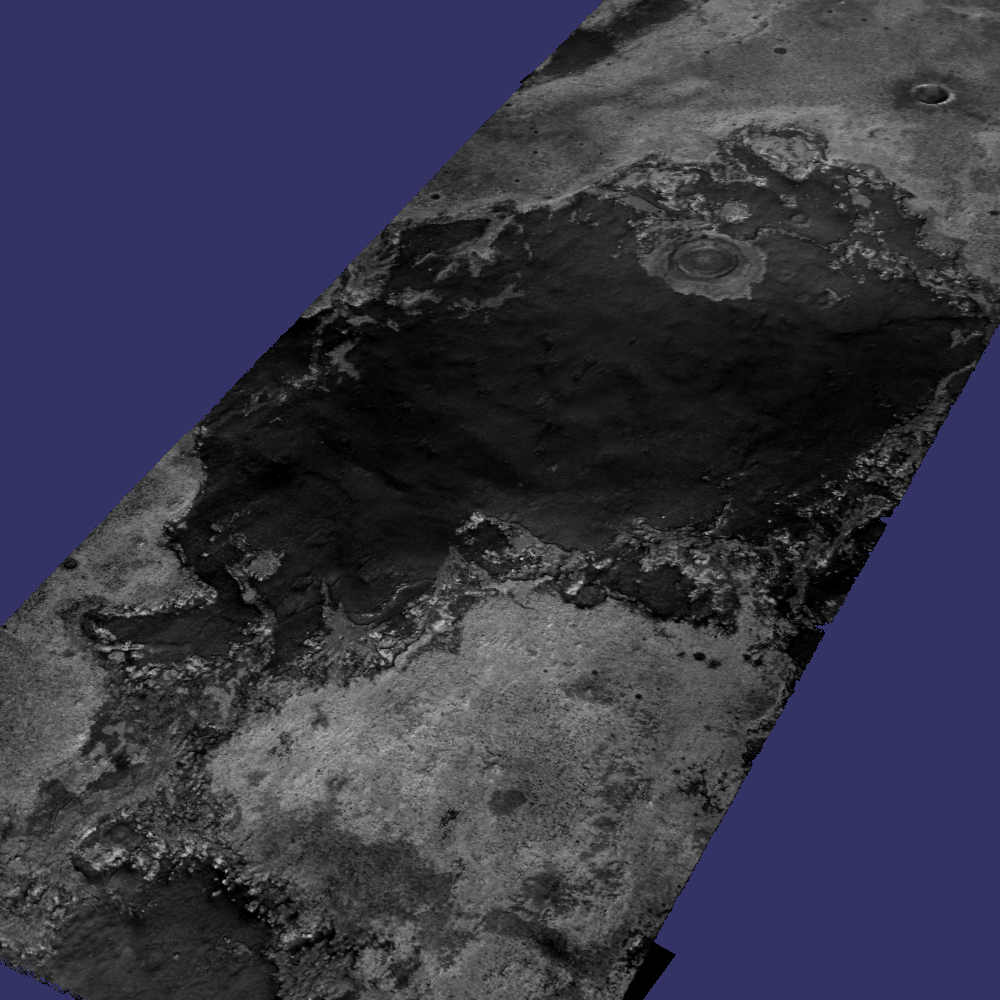
\includegraphics[width=3in]{images/examples/ctx/n_terra_meridiani_ctx.png}}
  \hfil
  \subfigure[{\tt KML Screenshot}]{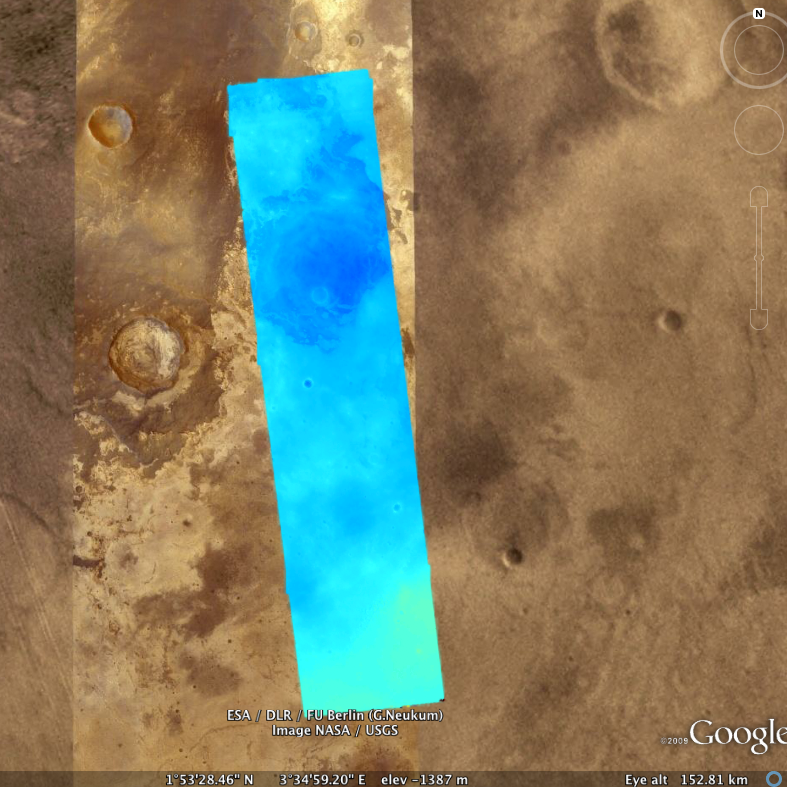
\includegraphics[width=3in]{images/examples/ctx/n_terra_meridiani_ctx_ge.png}}
\caption{Example output possible with the CTX imager aboard MRO.}
\label{fig:ctx_example}
\end{figure}

\subsubsection*{Commands}

Download the \ac{CTX} images P02\_001981\_1823\_XI\_02N356W.IMG and
P03\_002258\_1817\_XI\_01N356W.IMG from the \ac{PDS}.
\begin{verbatim}
  ISIS 3> mroctx2isis from=P02_001981_1823_XI_02N356W.IMG to=P02_001981_1823.cub
  ISIS 3> mroctx2isis from=P03_002258_1817_XI_01N356W.IMG to=P03_002258_1817.cub
  ISIS 3> spiceinit from=P02_001981_1823.cub
  ISIS 3> spiceinit from=P03_002258_1817.cub
  ISIS 3> ctxcal from=P02_001981_1823.cub to=P02_001981_1823.cal.cub
  ISIS 3> ctxcal from=P03_002258_1817.cub to=P03_002258_1817.cal.cub
  ISIS 3> cam2map from=P02_001981_1823.cal.cub to=P02_001981_1823.map.cub
  ISIS 3> cam2map from=P03_002258_1817.cal.cub to=P03_002258_1817.map.cub
  ISIS 3> mkdir result
  ISIS 3> stereo P02_001981_1823.map.cub P03_002258_1817.map.cub results/out
\end{verbatim}

\vfill

\subsubsection*{stereo.default}

\begin{center}\begin{minipage}{5.5in}
\begin{Verbatim}[frame=single,fontsize=\small,label=stereo.default for CTX North Terra Meridiani]
    ### PREPROCESSING

    DO_INTERESTPOINT_ALIGNMENT 1
    INTERESTPOINT_ALIGNMENT_SUBSAMPLING 0
    DO_EPIPOLAR_ALIGNMENT 0

    FORCE_USE_ENTIRE_RANGE 0
    DO_INDIVIDUAL_NORMALIZATION 0

    PREPROCESSING_FILTER_MODE 3

    SLOG_KERNEL_WIDTH 1.5

    ### CORRELATION

    COST_BLUR 0
    COST_MODE 2

    H_KERNEL 35
    V_KERNEL 35

    H_CORR_MIN -300
    H_CORR_MAX 300
    V_CORR_MIN -150
    V_CORR_MAX 150

    SUBPIXEL_MODE 3

    SUBPIXEL_H_KERNEL 21
    SUBPIXEL_V_KERNEL 21

    ### FILTERING

    FILL_HOLES 1

    RM_H_HALF_KERN 5
    RM_V_HALF_KERN 5
    RM_MIN_MATCHES 60 # Units = percent
    RM_THRESHOLD 3
    RM_CLEANUP_PASSES 1

    ### DOTCLOUD

    NEAR_UNIVERSE_RADIUS 0.0
    FAR_UNIVERSE_RADIUS 0.0
\end{Verbatim}
\end{minipage}\end{center}

\section{Mars Global Surveyor MOC-NA}

In the Stereo Pipeline Tutorial in Chapter~\ref{ch:tutorial}, we
showed you how to process a narrow angle \ac{MOC} stereo pair that
covered a portion of Hrad Vallis. In this section we will show you
more examples, some of which exhibit a problem common to stereo
pairs from linescan imagers: ``spacecraft jitter'' is caused by
oscillations of the spacecraft due to the movement of other spacecraft
hardware.  All spacecraft wobble around to some degree but some,
especially Mars Global Surveyor, are particularly susceptible.

Jitter causes wave-like distortions along the track of the satellite
orbit in \acp{DEM} produced from linescan camera images.  This effect can
be very subtle or quite pronounced, so it is important to check your
data products carefully for any sign of this type of artifact. The
following examples will show the typical distortions created by this
problem.

Note that the science teams of \ac{HiRISE} and \ac{LROC} are actively
working on detecting and correctly modeling jitter in their respective
SPICE data. If they succeed in this, the distortions will still
be present in the raw imagery, but the jitter will no longer produce
ripple artifacts in the DEMs produced using ours or other stereo
reconstruction software.

\subsection{Ceraunius Tholus}

Ceraunius Tholus is a volcano in northern Tharsis on Mars. It can
be found at 23.96 N and 262.60 E. This \ac{DEM} crosses the volcano's
caldera.

\begin{figure}[h!]
\centering
  \subfigure[{\tt 3D Rendering}]{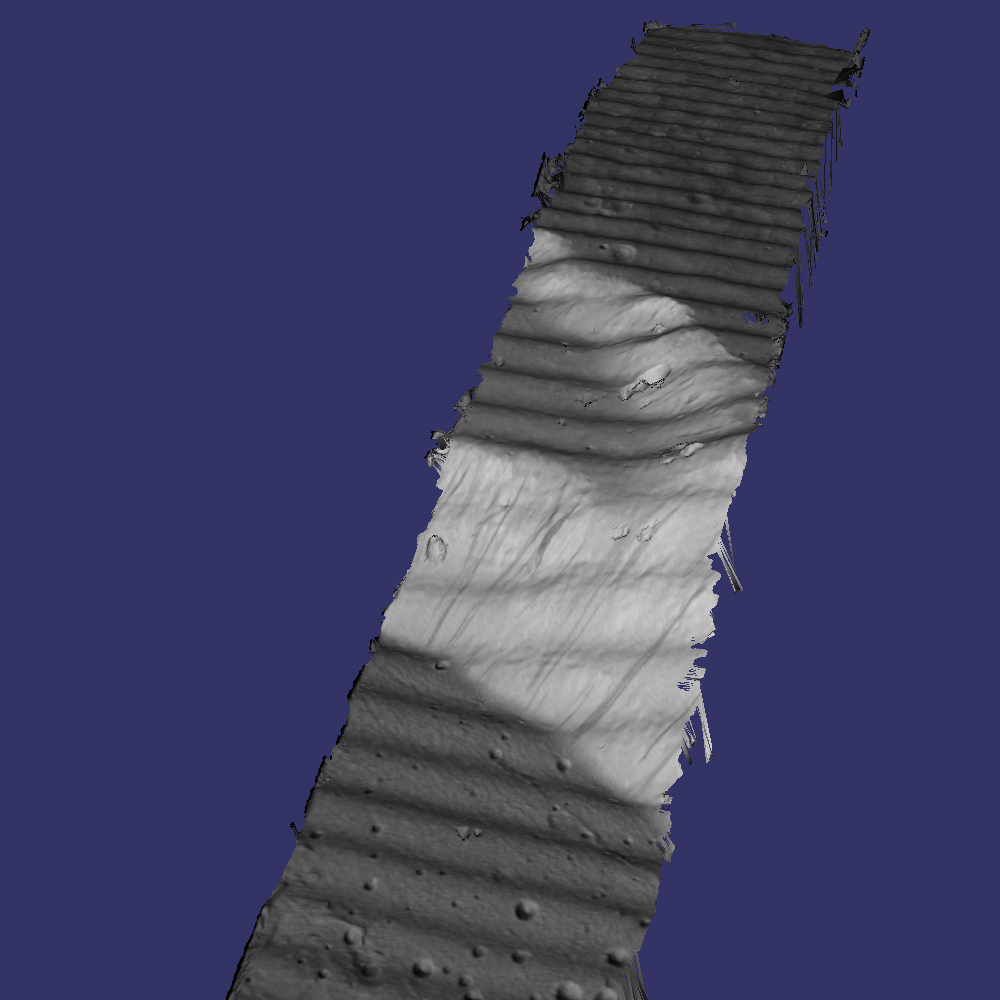
\includegraphics[width=3in]{images/examples/mocna/ceraunius_tholus_mocna.png}}
  \hfil
  \subfigure[{\tt KML Screenshot}]{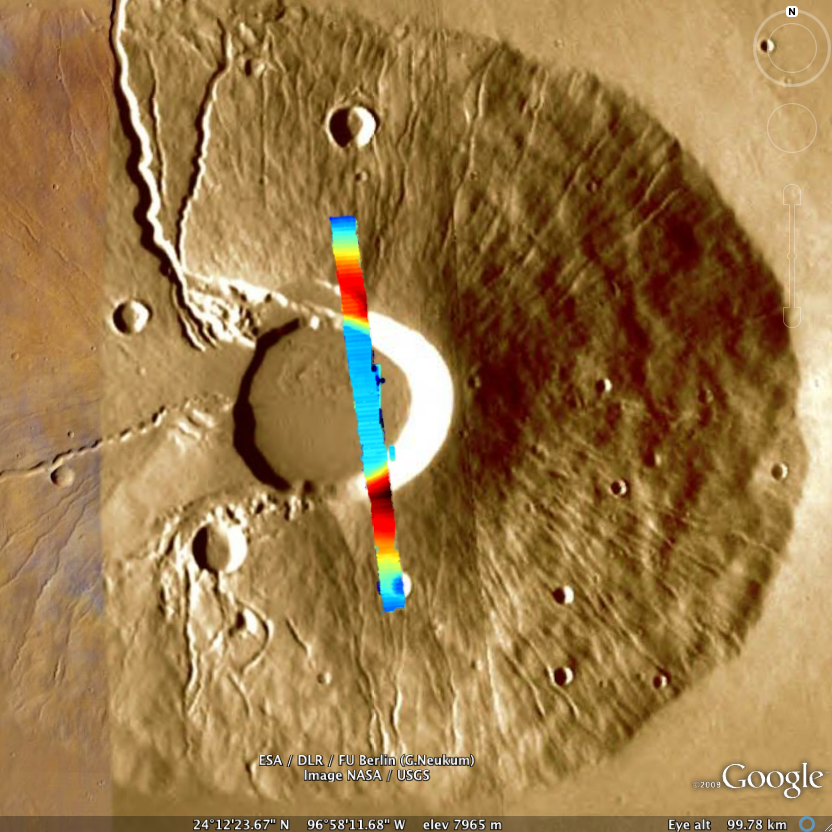
\includegraphics[width=3in]{images/examples/mocna/ceraunius_tholus_mocna_ge.png}}
\caption{Example output for MOC-NA of Ceraunius Tholus. Notice the presence of severe washboarding artifacts due to spacecraft ``jitter.''}
\label{fig:mocna_ceraunius_example}
\end{figure}

\subsubsection*{Commands}

Download the M08/06047 and R07/01361 images from the \ac{PDS}.
\begin{verbatim}
  ISIS 3> moc2isis f=M0806047.img t=M0806047.cub mapping=no
  ISIS 3> moc2isis f=R0701361.img t=R0701361.cub mapping=no
  ISIS 3> cam2map from=M0806047.cub to=M0806047.map.cub
  ISIS 3> cam2map from=R0701361.cub map=M0806047.map.cub to=R0701361.map.cub matchmap=true
  ISIS 3> mkdir result
  ISIS 3> stereo M0806047.map.cub R0701361.map.cub result/output
\end{verbatim}

\subsubsection*{stereo.default}

\begin{center}\begin{minipage}{5.5in}
\begin{Verbatim}[frame=single,fontsize=\small,label=stereo.default for MOC Ceraunius Tholus]
    ### PREPROCESSING

    DO_INTERESTPOINT_ALIGNMENT 0
    INTERESTPOINT_ALIGNMENT_SUBSAMPLING 0
    DO_EPIPOLAR_ALIGNMENT 0

    FORCE_USE_ENTIRE_RANGE 1
    DO_INDIVIDUAL_NORMALIZATION 1

    PREPROCESSING_FILTER_MODE 2

    SLOG_KERNEL_WIDTH 1.5

    ### CORRELATION

    COST_BLUR 12
    COST_MODE 2

    H_KERNEL 25
    V_KERNEL 25

    H_CORR_MIN -12
    H_CORR_MAX 26
    V_CORR_MIN -50
    V_CORR_MAX 15

    SUBPIXEL_MODE 2

    SUBPIXEL_H_KERNEL 21
    SUBPIXEL_V_KERNEL 21

    ### FILTERING

    FILL_HOLES 1

    RM_H_HALF_KERN 5
    RM_V_HALF_KERN 5
    RM_MIN_MATCHES 60 # Units = percent
    RM_THRESHOLD 3
    RM_CLEANUP_PASSES 1

    ### DOTCLOUD

    NEAR_UNIVERSE_RADIUS 0.0
    FAR_UNIVERSE_RADIUS 0.0
\end{Verbatim}
\end{minipage}\end{center}

\pagebreak
\subsection{North Tharsis}

These images cover troughs and terraces in northern Tharsis. 
This \ac{DEM} is located at 20.20 N and 118.18 W on Mars.

\begin{figure}[h!]
\centering
  \subfigure[{\tt 3D Rendering}]{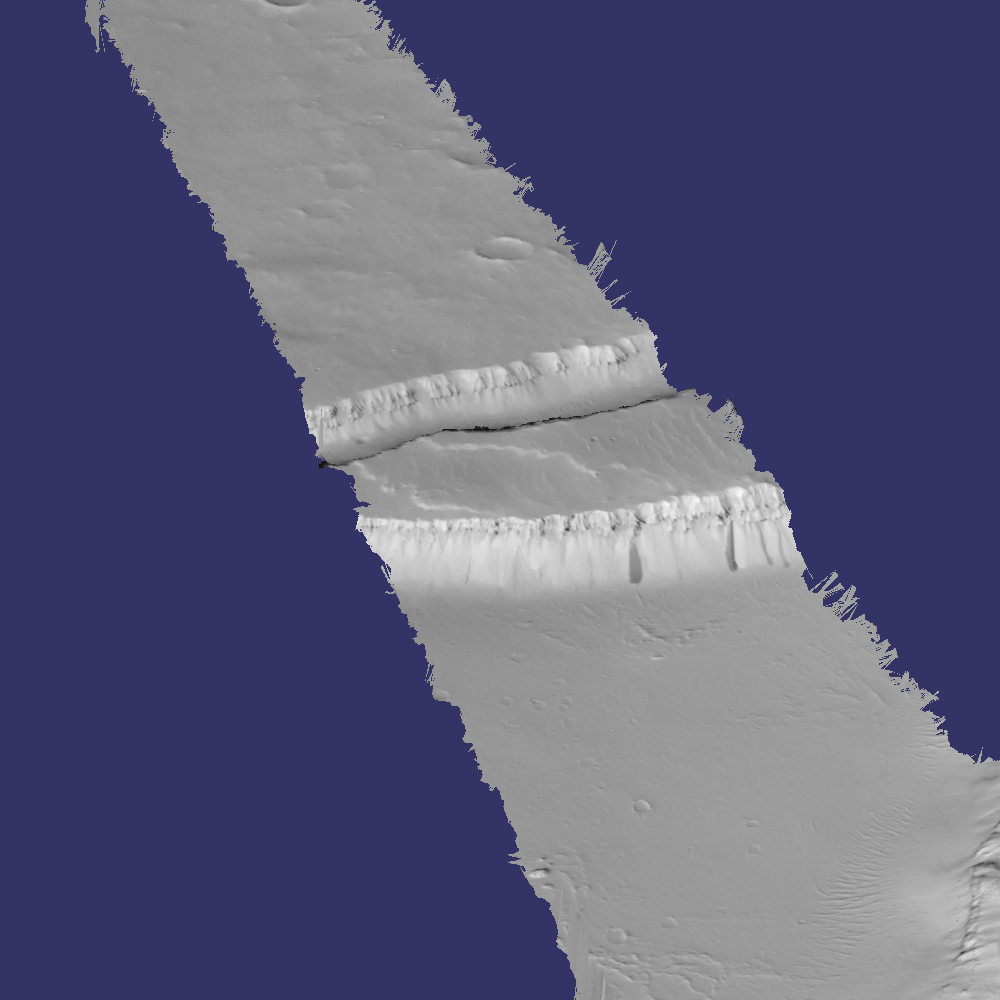
\includegraphics[width=3in]{images/examples/mocna/n_tharsis_mocna.png}}
  \hfil
  \subfigure[{\tt KML Screenshot}]{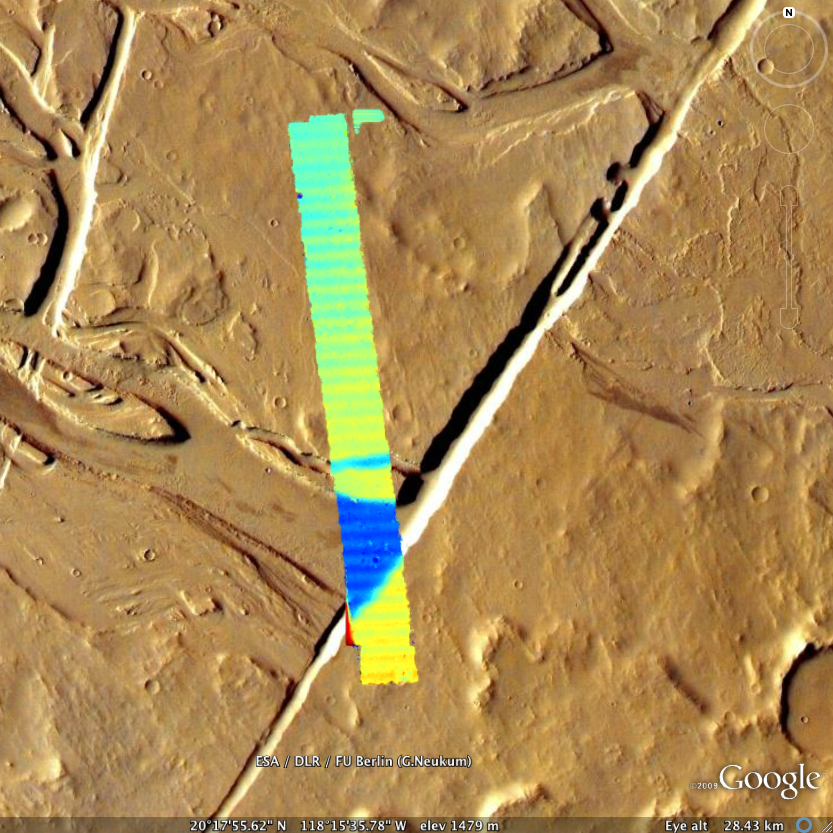
\includegraphics[width=3in]{images/examples/mocna/n_tharsis_mocna_ge.png}}
\caption{Example output for MOC-NA of North Tharsis.}
\label{fig:mocna_n_tharsis_example}
\end{figure}

\subsubsection*{Commands}

Download the M08/03097.img and S07/01420 images from the \ac{PDS}.
\begin{verbatim}
  ISIS 3> moc2isis f=M0803097.img t=M0803097.cub mapping=no
  ISIS 3> moc2isis f=S0701420.img t=S0701420.cub mapping=no
  ISIS 3> cam2map from=M0803097.cub to=M0803097.map.cub
  ISIS 3> cam2map from=S0701420.cub map=M0803097.map.cub to=S0701420.map.cub matchmap=true
  ISIS 3> mkdir result
  ISIS 3> stereo M0803097.map.cub S0701420.map.cub result/output
\end{verbatim}

\vfill

\subsubsection*{stereo.default}

\begin{center}\begin{minipage}{5.5in}
\begin{Verbatim}[frame=single,fontsize=\small,label=stereo.default for MOC North Tharsis]
    ### PREPROCESSING

    DO_INTERESTPOINT_ALIGNMENT 0
    INTERESTPOINT_ALIGNMENT_SUBSAMPLING 0
    DO_EPIPOLAR_ALIGNMENT 0

    FORCE_USE_ENTIRE_RANGE 1
    DO_INDIVIDUAL_NORMALIZATION 1

    PREPROCESSING_FILTER_MODE 2

    SLOG_KERNEL_WIDTH 1.5

    ### CORRELATION

    COST_BLUR 12
    COST_MODE 2

    H_KERNEL 25
    V_KERNEL 25

    H_CORR_MIN -50
    H_CORR_MAX 0
    V_CORR_MIN -85
    V_CORR_MAX 0

    SUBPIXEL_MODE 2

    SUBPIXEL_H_KERNEL 21
    SUBPIXEL_V_KERNEL 21

    ### FILTERING

    FILL_HOLES 1

    RM_H_HALF_KERN 5
    RM_V_HALF_KERN 5
    RM_MIN_MATCHES 60 # Units = percent
    RM_THRESHOLD 3
    RM_CLEANUP_PASSES 1

    ### DOTCLOUD

    NEAR_UNIVERSE_RADIUS 0.0
    FAR_UNIVERSE_RADIUS 0.0
\end{Verbatim}
\end{minipage}\end{center}

\section{Lunar Reconaissance Orbiter LROC NAC}

When \ac{LROC} image data are released, map projection processes
very similar to those run on other linescan imagers can be used.
The example \texttt{stereo.default} file would be a good place to
start from, as well.

% \subsection{Lee-Lincoln Scarp}
% 
% This stereo pair covers the Taurus-Littrow valley on the Moon where,
% on December 11, 1972, the astronauts of Apollo 17 landed. However,
% this stereo pair does not contain the landing site.  It is slightly
% west; focusing on the Lee-Lincoln scarp that is on North Massif. The
% scarp is an 80~m high feature that is the only visible sign of a deep
% fault.
% 
% \begin{figure}[h!]
% \centering
%   \subfigure[{\tt 3D Rendering}]{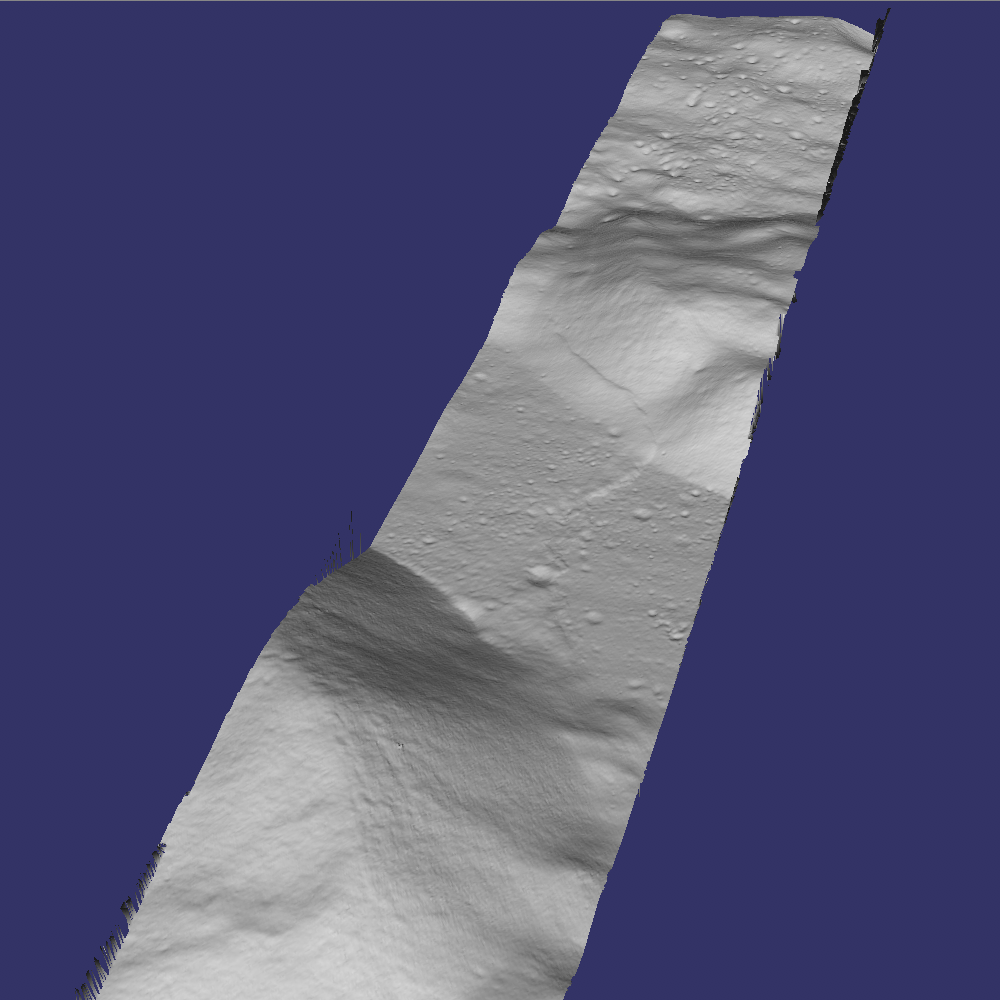
\includegraphics[width=3in]{images/examples/lrocna/lroc-na-example.png}}
%   \hfil
%   \subfigure[{\tt KML Screenshot}]{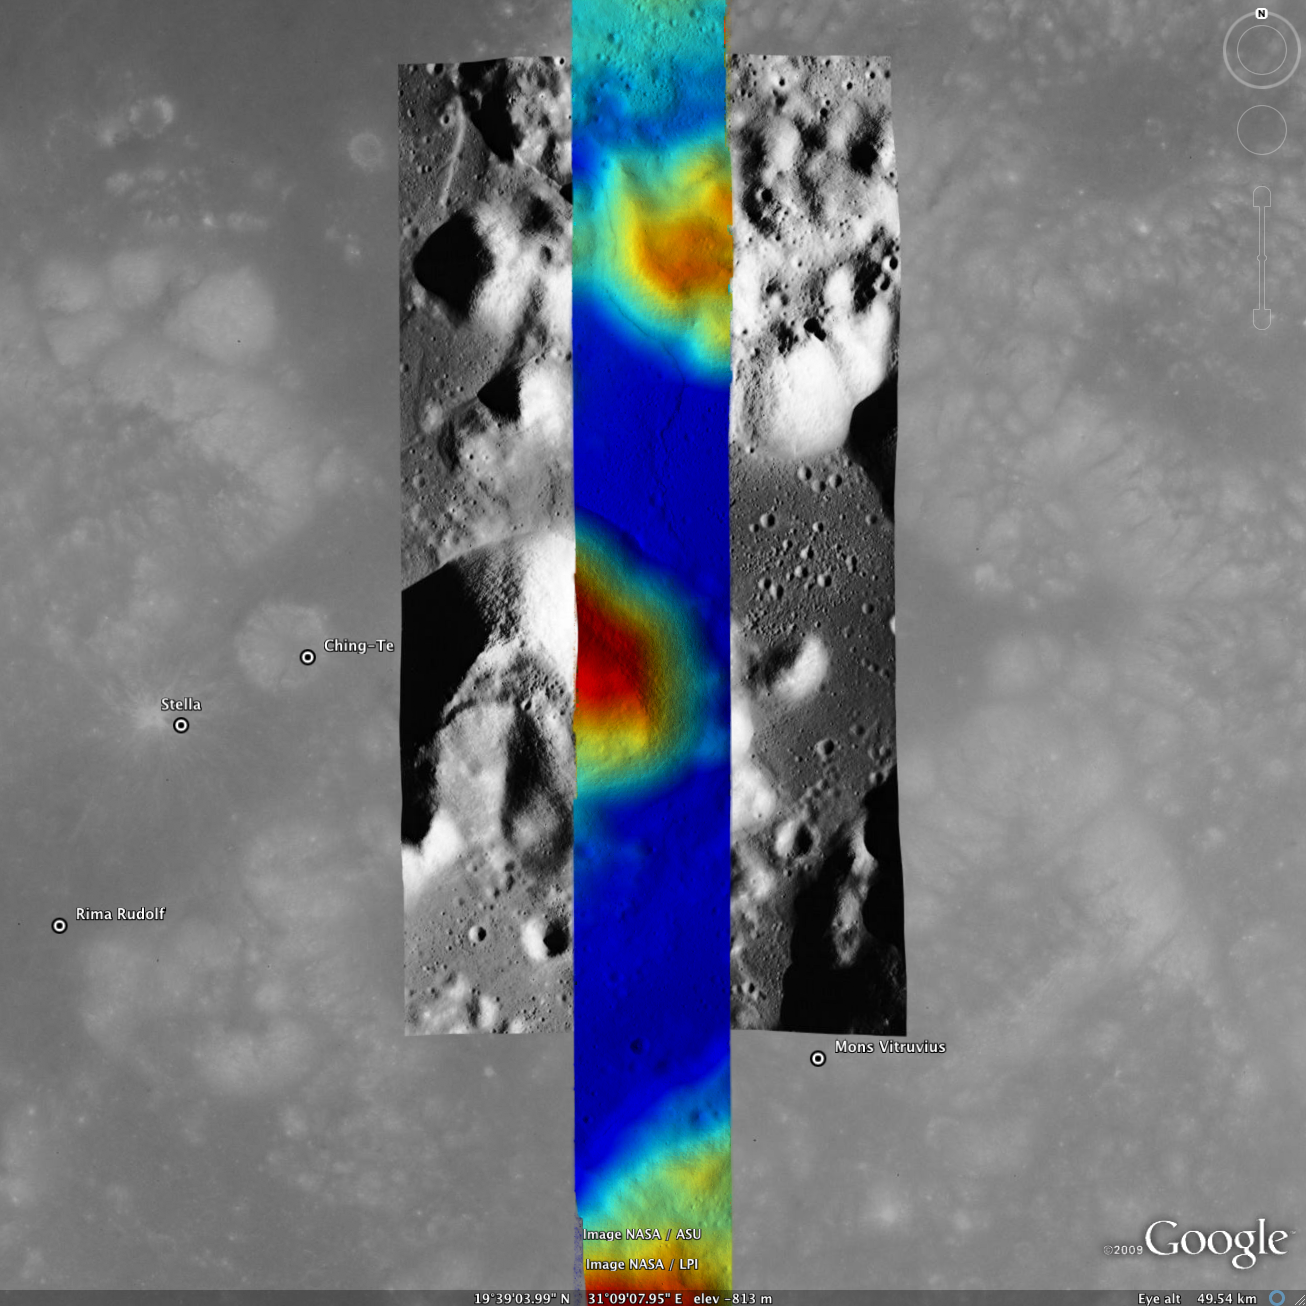
\includegraphics[width=3in]{images/examples/lrocna/lroc-na-ge_example.png}}
% \caption{Example output possible with a LROC NA stereo pair, using only a single CCDs from observations.}
% \label{fig:lroc-na-example}
% \end{figure}

\subsubsection*{Commands}

\begin{verbatim}
    ISIS 3> cam2map from=lroc-1sthalf.cub to=lroc-1sthalf.map.cub
    ISIS 3> cam2map from=lroc-2ndhalf.cub map=lroc-2ndhalf.map.cub \
                    to=lroc-1sthalf.map.cub matchmap=true
    ISIS 3> mkdir result
    ISIS 3> stereo lroc-1sthalf.map.cub lroc-2ndhalf.map.cub result/output
\end{verbatim}

\subsubsection*{stereo.default}

\begin{center}\begin{minipage}{5.5in}
\begin{Verbatim}[frame=single,fontsize=\small,label=stereo.default for LROC NAC]
    ### PREPROCESSING

    DO_INTERESTPOINT_ALIGNMENT 0
    INTERESTPOINT_ALIGNMENT_SUBSAMPLING 0
    DO_EPIPOLAR_ALIGNMENT 0

    FORCE_USE_ENTIRE_RANGE 1
    DO_INDIVIDUAL_NORMALIZATION 0

    PREPROCESSING_FILTER_MODE 2

    SLOG_KERNEL_WIDTH 1.5

    ### CORRELATION

    COST_BLUR 12
    COST_MODE 2

    H_KERNEL 29
    V_KERNEL 29

    H_CORR_MIN -425
    H_CORR_MAX 150
    V_CORR_MIN -100
    V_CORR_MAX 100

    SUBPIXEL_MODE 2

    SUBPIXEL_H_KERNEL 25
    SUBPIXEL_V_KERNEL 25

    ### FILTERING

    FILL_HOLES 1

    RM_H_HALF_KERN 5
    RM_V_HALF_KERN 5
    RM_MIN_MATCHES 60 # Units = percent
    RM_THRESHOLD 3
    RM_CLEANUP_PASSES 1

    ### DOTCLOUD

    NEAR_UNIVERSE_RADIUS 0.0
    FAR_UNIVERSE_RADIUS 0.0
\end{Verbatim}
\end{minipage}\end{center}

\section{Apollo 15 Metric Camera Images}

Apollo Metric images were all taken at regular intervals, which means
that the same \texttt{stereo.default} can be used for all sequential pairs of
images. Apollo Metric images are ideal for stereo processing.  They
produce consistent, excellent results.

The scans performed by ASU are sufficiently detailed to exhibit film
grain at the highest resolution.  The amount of noise at the full
resolution is not helpful for the correlator, so we recommended
subsampling the images by a factor of 4.

Currently the tools to ingest Apollo TIFFs into ISIS are not
available, but these images should soon be released into the PDS for
general public usage.

\subsection{Ansgarius C}

Ansgarius C is a small crater on the west edge of the farside of the
Moon near the equator. It is east of Kapteyn A and B.

\begin{figure}[h!]
\centering
  \subfigure[{\tt 3D Rendering}]{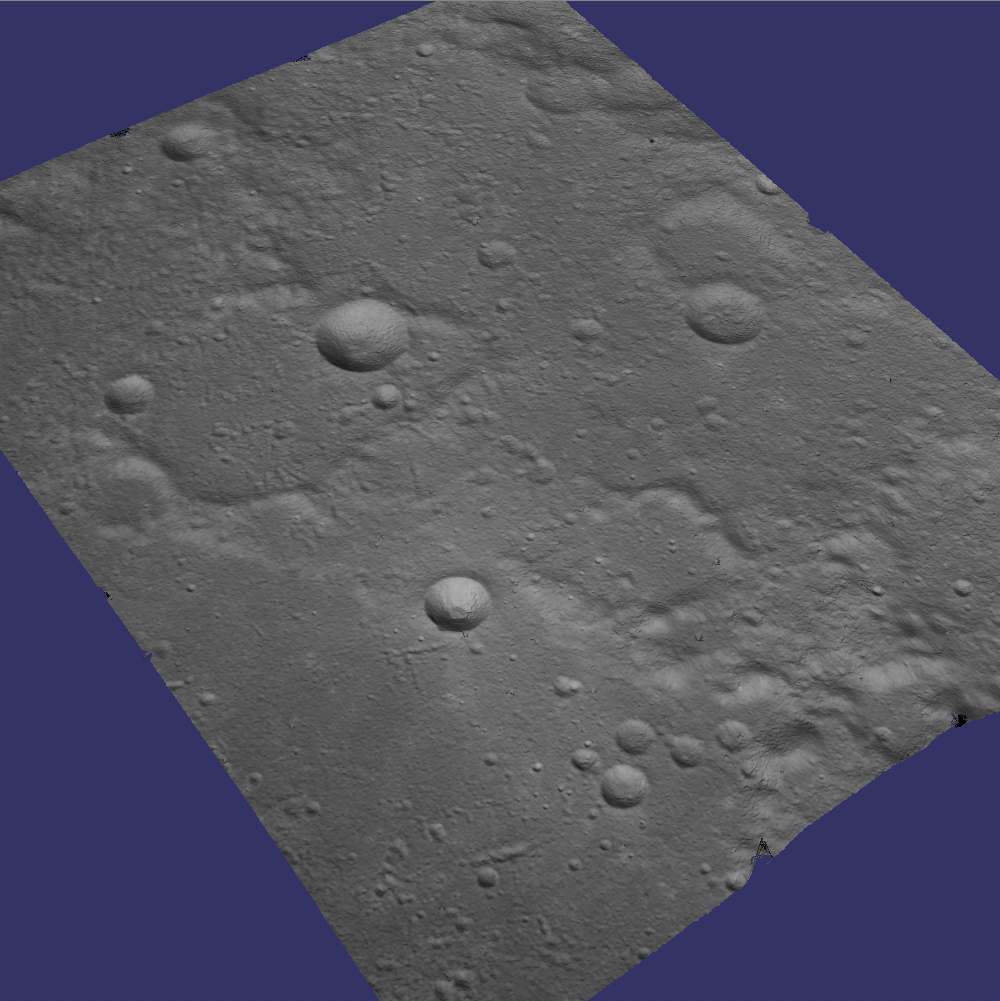
\includegraphics[width=3in]{images/examples/metric/metric_example.png}}
  \hfil
  \subfigure[{\tt KML Screenshot}]{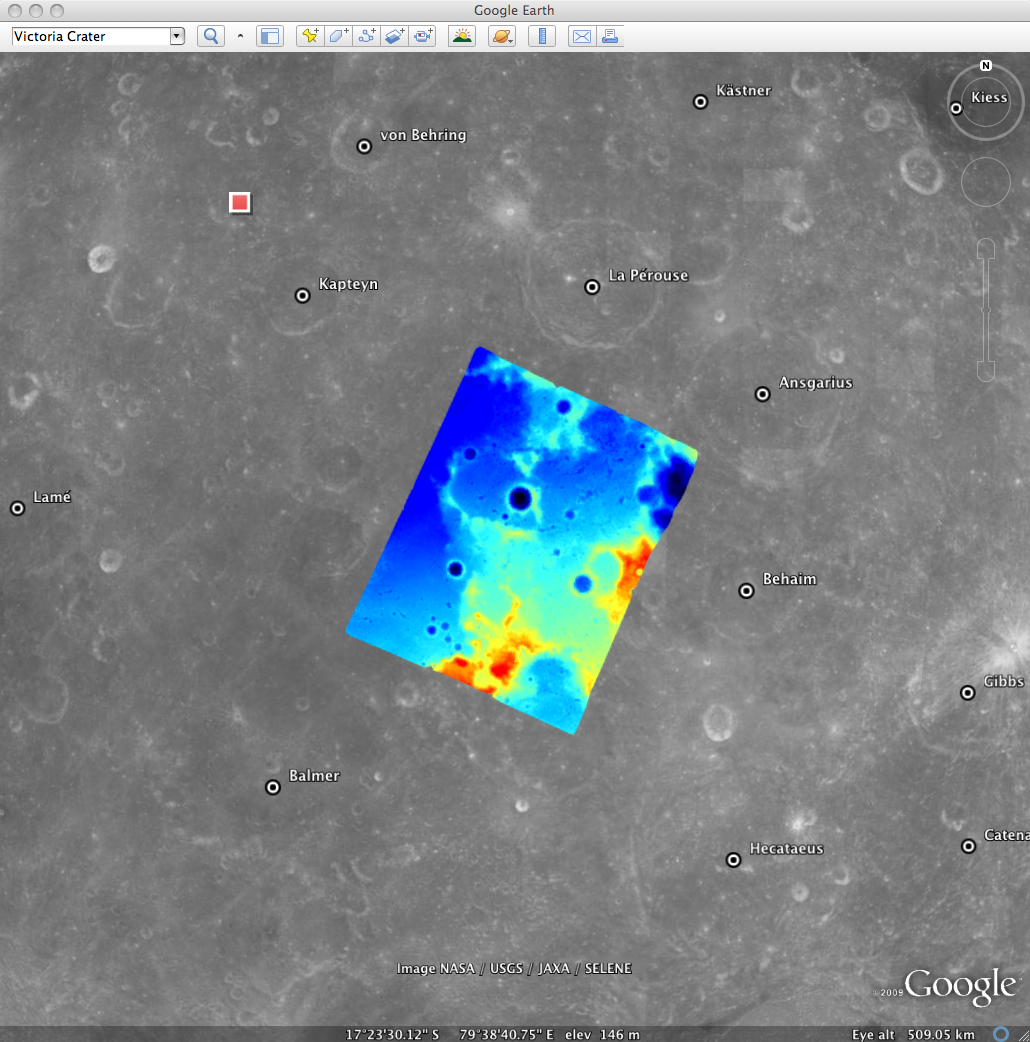
\includegraphics[width=3in]{images/examples/metric/metric_ge_example.png}}
\caption{Example output possible with Apollo Metric frames AS15-M-2380 and AS15-M-2381.}
\label{fig:metric_example}
\end{figure}

\subsubsection*{Commands}

Process Apollo TIFF files into \ac{ISIS}.
\begin{verbatim}
  ISIS 3> reduce from=AS15-M-2380.cub to=sub4-AS15-M-2380.cub sscale=4 lscale=4
  ISIS 3> reduce from=AS15-M-2381.cub to=sub4-AS15-M-2381.cub sscale=4 lscale=4
  ISIS 3> spiceinit from=sub4-AS15-M-2380.cub
  ISIS 3> spiceinit from=sub4-AS15-M-2381.cub
  ISIS 3> ipfind --max 10000 sub4*.cub
  ISIS 3> ipmatch -i 50 -r homography sub4*.cub
  ISIS 3> mkdir result
  ISIS 3> stereo sub4-AS15-M-2380.cub sub4-AS15-M-2381.cub result/output
\end{verbatim}

\subsubsection*{stereo.default}

\begin{center}\begin{minipage}{5.5in}
\begin{Verbatim}[frame=single,fontsize=\small,label=stereo.default for Apollo 15 Metric Camera]
    ### PREPROCESSING

    DO_INTERESTPOINT_ALIGNMENT 1
    INTERESTPOINT_ALIGNMENT_SUBSAMPLING 0
    DO_EPIPOLAR_ALIGNMENT 0

    FORCE_USE_ENTIRE_RANGE 1
    DO_INDIVIDUAL_NORMALIZATION 0

    PREPROCESSING_FILTER_MODE 3

    SLOG_KERNEL_WIDTH 1.5

    ### CORRELATION

    COST_MODE 2
    COST_BLUR 25

    H_KERNEL 35
    V_KERNEL 35

    H_CORR_MIN -250
    H_CORR_MAX 250
    V_CORR_MIN -70
    V_CORR_MAX 100

    SUBPIXEL_MODE 2

    SUBPIXEL_H_KERNEL 25
    SUBPIXEL_V_KERNEL 25

    # Hidden advanced function
    CORRSCORE_REJECTION_THRESHOLD 1.4

    ### FILTERING

    FILL_HOLES 1

    RM_H_HALF_KERN 5
    RM_V_HALF_KERN 5
    RM_MIN_MATCHES 60 # Units = percent
    RM_THRESHOLD 3
    RM_CLEANUP_PASSES 1

    ### DOTCLOUD

    NEAR_UNIVERSE_RADIUS 0.0
    FAR_UNIVERSE_RADIUS 0.0
\end{Verbatim}
\end{minipage}\end{center}

\section{MESSENGER MDIS}

These results are a proof of concept showing off the strength of
building the Stereo Pipeline on top of \ac{ISIS}. Support for processing
MDIS stereo pairs was not a goal during our design of the software,
but the fact that an MDIS camera model exists in ISIS means that
it too can be processed by the Stereo Pipeline.

For future mappers, we suggest checking out Mercury Flyby 3 data which
was not available at the time of this writing. Flyby 3 and Flyby 2
seem to have covered some of the same terrain with the narrow angle
camera.

\subsection{Wide Angle on flyby 2}

In most flyby imagery it is very hard to find good stereo pairs.
This pair was taken from a single flyby just seconds apart. Note
also that this pair is taken from different wavelengths (the letter
at the end of the filename designates the current filter being used
on the wide angle camera). Unfortunately there is not enough of a
perspective change here to make anything other than the spherical
surface, but that alone is still an interesting result nonetheless.

\begin{figure}[h!]
  \begin{center}
  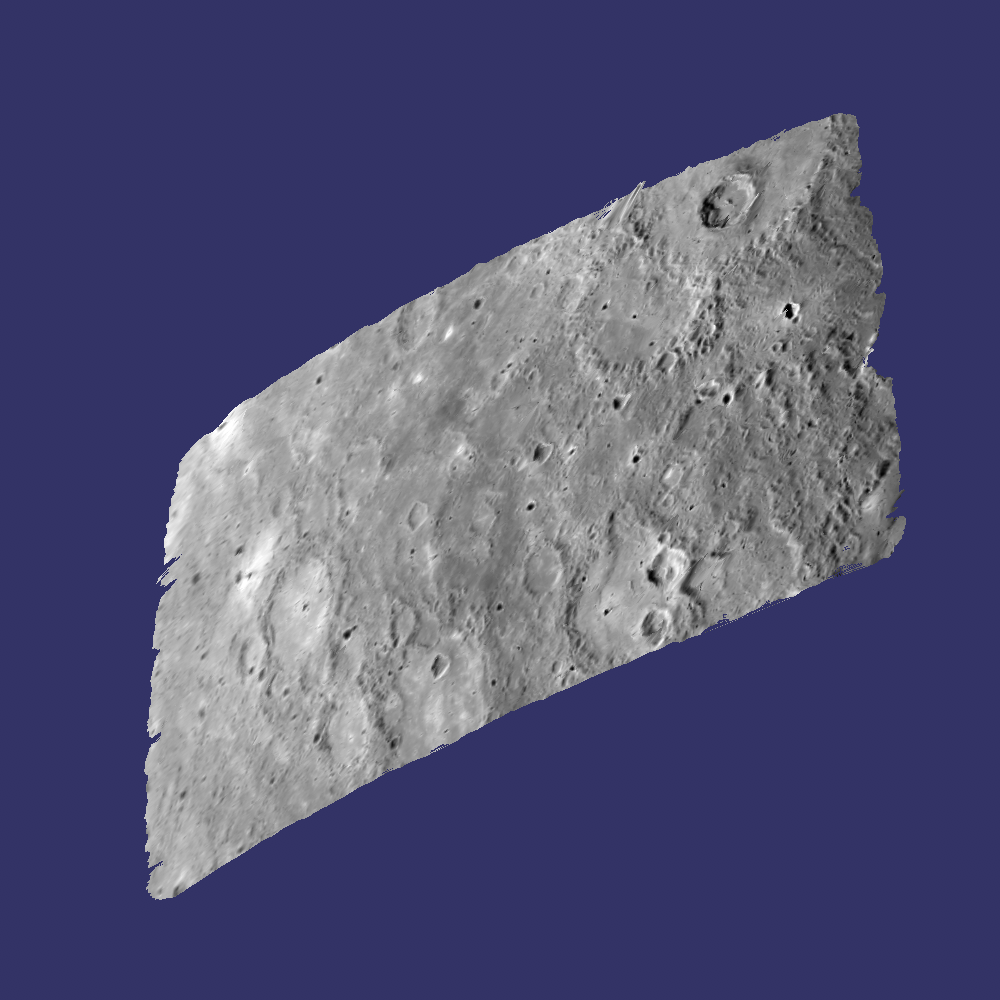
\includegraphics[width=5in]{images/examples/mdis/mdis_wide_example.png}
  \end{center}
  \caption{ A rough attempt at stereo reconstruction from MDIS imagery. }
  \label{fig:mdis_attempt}
\end{figure}

\subsubsection*{Commands}

\begin{verbatim}
  ISIS 3> mdis2isis from=EW0108825359A.IMG to=EW0108825359A.cub
  ISIS 3> mdis2isis from=EW0108825379C.IMG to=EW0108825379C.cub
  ISIS 3> spiceinit from=EW0108825359A.cub
  ISIS 3> spiceinit from=EW0108825359C.cub
  ISIS 3> ipfind --max 10000 *.cub
  ISIS 3> ipmatch -i 10 -r homography *.cub
  ISIS 3> mkdir result
  ISIS 3> stereo EW0108825359A.cub EW0108825379C.cub stereo/output
\end{verbatim}

\subsubsection*{stereo.default}

\begin{center}\begin{minipage}{5.5in}
\begin{Verbatim}[frame=single,fontsize=\small,label=stereo.default for MDIS]
    ### PREPROCESSING

    DO_INTERESTPOINT_ALIGNMENT 1
    INTERESTPOINT_ALIGNMENT_SUBSAMPLING 0
    DO_EPIPOLAR_ALIGNMENT 0

    FORCE_USE_ENTIRE_RANGE 0
    DO_INDIVIDUAL_NORMALIZATION 1

    PREPROCESSING_FILTER_MODE 2

    SLOG_KERNEL_WIDTH 1.5

    ### CORRELATION

    COST_BLUR 5
    COST_MODE 0

    H_KERNEL 25
    V_KERNEL 25

    H_CORR_MIN -10
    H_CORR_MAX 10
    V_CORR_MIN -2
    V_CORR_MAX 2

    SUBPIXEL_MODE 2

    SUBPIXEL_H_KERNEL 19
    SUBPIXEL_V_KERNEL 19

    ### FILTERING

    FILL_HOLES 1

    RM_H_HALF_KERN 5
    RM_V_HALF_KERN 5
    RM_MIN_MATCHES 60 # Units = percent
    RM_THRESHOLD 3
    RM_CLEANUP_PASSES 1

    ### DOTCLOUD

    NEAR_UNIVERSE_RADIUS 0.0
    FAR_UNIVERSE_RADIUS 0.0
\end{Verbatim}
\end{minipage}\end{center}

\section{Cassini ISS NAC}

This is a proof of concept showing the strength of building the Stereo
Pipeline on top of \ac{ISIS}.  Support for processing ISS NAC stereo pairs
was not a goal during our design of the software, but the fact that a
camera model exists in \ac{ISIS} means that it too can be processed by the
Stereo Pipeline.

Identifying stereo pairs from spacecraft that do not orbit their
target is a challenge. We have found that one usually has to settle
with images that are not ideal: different lighting, little perspective
change, and little or no stereo parallax. So far we have had little
success with Cassini's data, but nonetheless we provide this example
as a potential starting point.

\subsection{Rhea}

Rhea is the second largest moon of Saturn and is roughly a third the
size of our own Moon. This example shows, at the top right of both
images,a giant impact basin named Tirawa that is 220~miles across. The
bright white area south of Tirawa is ejecta from a new crater.  The
lack of texture in this area poses a challenge for our correlator. The
results are just barely useful: the Tirawa impact can barely be made
out in the 3D data while the new crater and ejecta become only noise.

\begin{figure}[p]
\centering
  \subfigure[{\tt Original Left Image}]{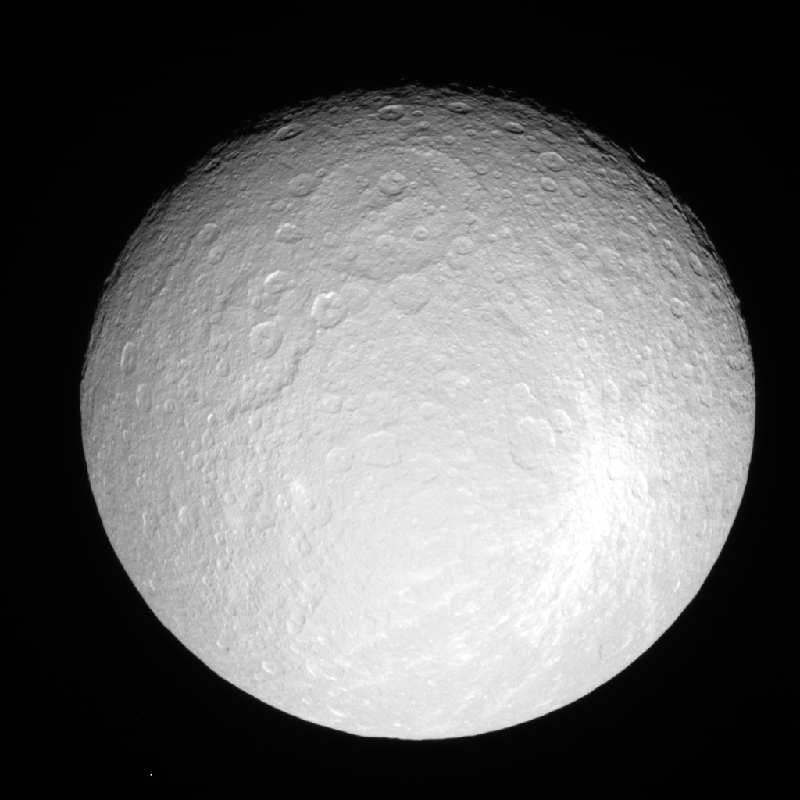
\includegraphics[width=3in]{images/examples/cassini/cassini_rhea_L.png}}
  \hfil
  \subfigure[{\tt Original Right Image}]{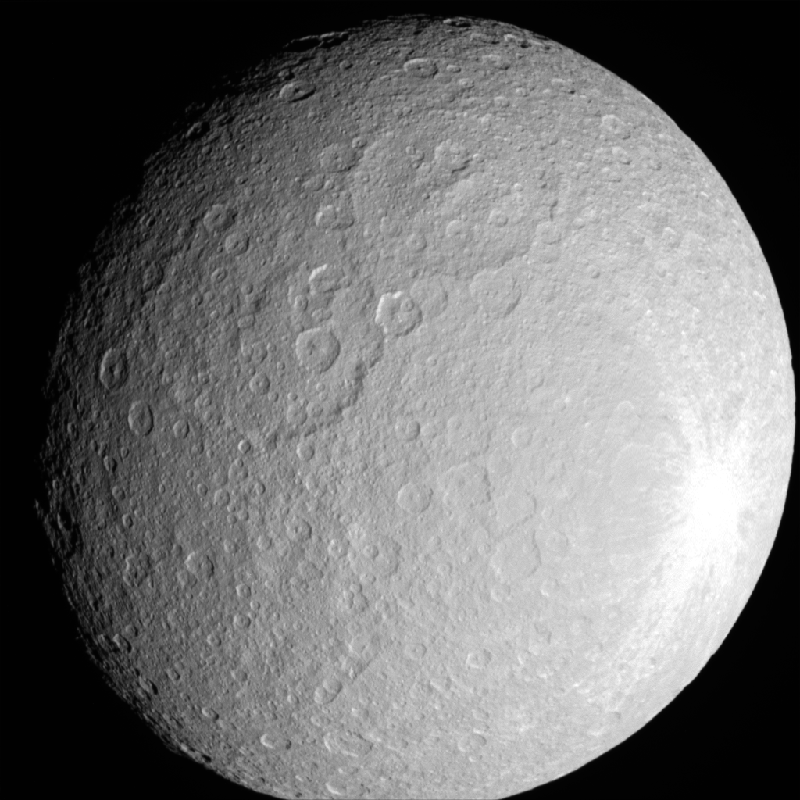
\includegraphics[width=3in]{images/examples/cassini/cassini_rhea_R.png}}
  \\
  \subfigure[{\tt Map Projected Left}]{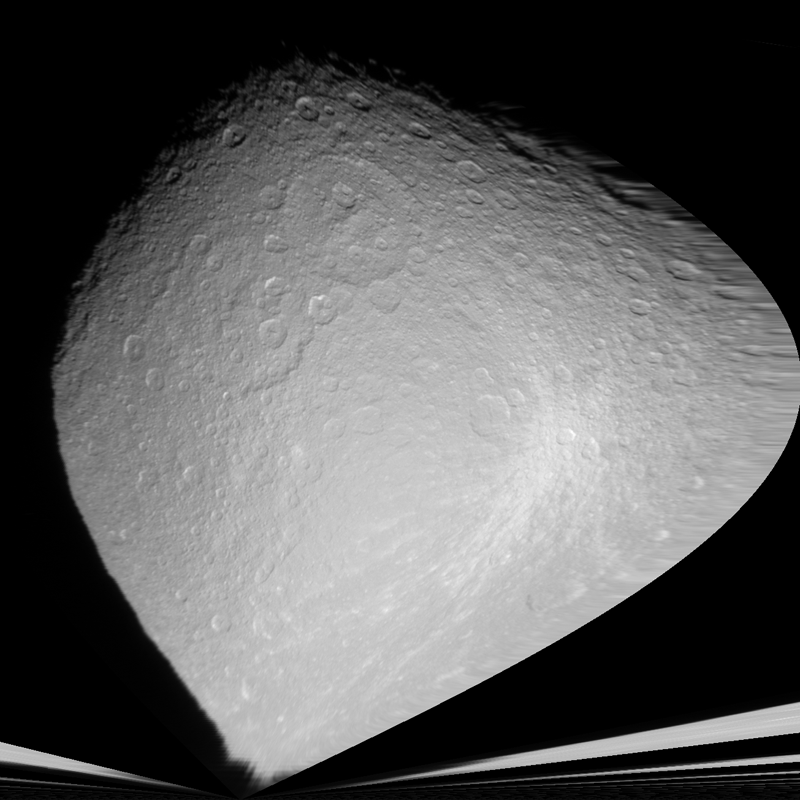
\includegraphics[width=3in]{images/examples/cassini/cassini_rhea_map.png}}
  \hfil
  \subfigure[{\tt 3D Rendering}]{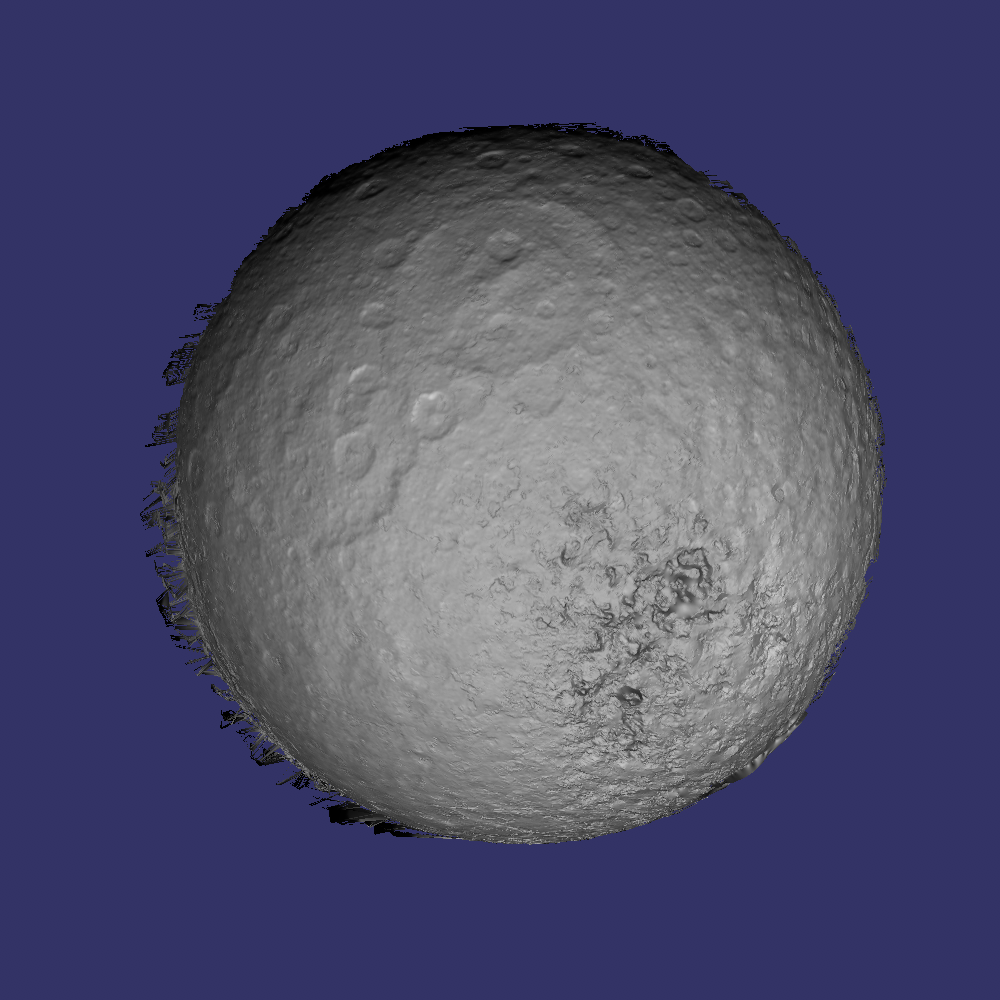
\includegraphics[width=3in]{images/examples/cassini/cassini_rhea.png}}
\caption{Example output of what is possible with Cassini's ISS NAC}
\label{fig:cassini-exampe}
\end{figure}

\subsubsection*{Commands}

Download the N1511700120\_1.IMG and W1567133629\_1.IMG images from the \ac{PDS}.
\begin{verbatim}
  ISIS 3> ciss2isis f=N1511700120_1.IMG t=N1511700120_1.cub
  ISIS 3> ciss2isis f=W1567133629_1.IMG t=W1567133629_1.cub
  ISIS 3> cisscal from=N1511700120_1.cub to=N1511700120_1.lev1.cub
  ISIS 3> cisscal from=W1567133629_1.cub to=W1567133629_1.lev1.cub
  ISIS 3> fillgap from=W1567133629_1.lev1.cub to=W1567133629_1.fill.cub %Only one image
                                                                        %exhibits the problem
  ISIS 3> cubenorm from=N1511700120_1.lev1.cub to=N1511700120_1.norm.cub
  ISIS 3> cubenorm from=W1567133629_1.fill.cub to=W1567133629_1.norm.cub
  ISIS 3> cam2map from=N1511700120_1.norm.cub to=N1511700120_1.map.cub
  ISIS 3> cam2map from=W1567133629_1.norm.cub map=N1511700120_1.map.cub \
  ISIS 3>           to=W1567133629_1.map.cub matchmap=true;
  ISIS 3> ls *.map.cub > fromlist
  ISIS 3> ls N*.map.cub > holdlist
  ISIS 3> equalizer fromlist=fromlist holdlist=holdlist
  ISIS 3> mkdir result
  ISIS 3> stereo N1511700120_1.map.equ.cub W1567133629_1.map.equ.cub result/rhea
\end{verbatim}

\subsubsection*{stereo.default}

\begin{center}\begin{minipage}{5.5in}
\begin{Verbatim}[frame=single,fontsize=\small,label=stereo.default for Cassini ISS]
    ### PREPROCESSING

    DO_INTERESTPOINT_ALIGNMENT 0
    INTERESTPOINT_ALIGNMENT_SUBSAMPLING 0
    DO_EPIPOLAR_ALIGNMENT 0

    FORCE_USE_ENTIRE_RANGE 1
    DO_INDIVIDUAL_NORMALIZATION 1

    PREPROCESSING_FILTER_MODE 2

    SLOG_KERNEL_WIDTH 1.5

    ### CORRELATION

    COST_MODE 2
    COST_BLUR 11

    H_KERNEL 25
    V_KERNEL 25

    H_CORR_MIN -55
    H_CORR_MAX -5
    V_CORR_MIN -2
    V_CORR_MAX 10

    SUBPIXEL_MODE 3 # Experimental Subpixel Mode

    SUBPIXEL_H_KERNEL 21
    SUBPIXEL_V_KERNEL 21

    ### FILTERING

    FILL_HOLES 1

    RM_H_HALF_KERN 5
    RM_V_HALF_KERN 5
    RM_MIN_MATCHES 60 # Units = percent
    RM_THRESHOLD 3
    RM_CLEANUP_PASSES 1

    ### DOTCLOUD

    NEAR_UNIVERSE_RADIUS 0.0
    FAR_UNIVERSE_RADIUS 0.0
\end{Verbatim}
\end{minipage}\end{center}
